\PassOptionsToPackage{unicode=true}{hyperref} % options for packages loaded elsewhere
\PassOptionsToPackage{hyphens}{url}
%
\documentclass[
  ignorenonframetext,
]{beamer}
\usepackage{pgfpages}
\setbeamertemplate{caption}[numbered]
\setbeamertemplate{caption label separator}{: }
\setbeamercolor{caption name}{fg=normal text.fg}
\beamertemplatenavigationsymbolsempty
% Prevent slide breaks in the middle of a paragraph:
\widowpenalties 1 10000
\raggedbottom
\setbeamertemplate{part page}{
  \centering
  \begin{beamercolorbox}[sep=16pt,center]{part title}
    \usebeamerfont{part title}\insertpart\par
  \end{beamercolorbox}
}
\setbeamertemplate{section page}{
  \centering
  \begin{beamercolorbox}[sep=12pt,center]{part title}
    \usebeamerfont{section title}\insertsection\par
  \end{beamercolorbox}
}
\setbeamertemplate{subsection page}{
  \centering
  \begin{beamercolorbox}[sep=8pt,center]{part title}
    \usebeamerfont{subsection title}\insertsubsection\par
  \end{beamercolorbox}
}
\AtBeginPart{
  \frame{\partpage}
}
\AtBeginSection{
  \ifbibliography
  \else
    \frame{\sectionpage}
  \fi
}
\AtBeginSubsection{
  \frame{\subsectionpage}
}
\usepackage{lmodern}
\usepackage{amssymb,amsmath}
\usepackage{ifxetex,ifluatex}
\ifnum 0\ifxetex 1\fi\ifluatex 1\fi=0 % if pdftex
  \usepackage[T1]{fontenc}
  \usepackage[utf8]{inputenc}
  \usepackage{textcomp} % provides euro and other symbols
\else % if luatex or xelatex
  \usepackage{unicode-math}
  \defaultfontfeatures{Scale=MatchLowercase}
  \defaultfontfeatures[\rmfamily]{Ligatures=TeX,Scale=1}
\fi
% use upquote if available, for straight quotes in verbatim environments
\IfFileExists{upquote.sty}{\usepackage{upquote}}{}
\IfFileExists{microtype.sty}{% use microtype if available
  \usepackage[]{microtype}
  \UseMicrotypeSet[protrusion]{basicmath} % disable protrusion for tt fonts
}{}
\makeatletter
\@ifundefined{KOMAClassName}{% if non-KOMA class
  \IfFileExists{parskip.sty}{%
    \usepackage{parskip}
  }{% else
    \setlength{\parindent}{0pt}
    \setlength{\parskip}{6pt plus 2pt minus 1pt}}
}{% if KOMA class
  \KOMAoptions{parskip=half}}
\makeatother
\usepackage{xcolor}
\IfFileExists{xurl.sty}{\usepackage{xurl}}{} % add URL line breaks if available
\IfFileExists{bookmark.sty}{\usepackage{bookmark}}{\usepackage{hyperref}}
\hypersetup{
  pdftitle={Variables locales et globales},
  pdfauthor={Ellie Tideswell and Jeremy Bornerieux},
  pdfborder={0 0 0},
  breaklinks=true}
\urlstyle{same}  % don't use monospace font for urls
\newif\ifbibliography
\usepackage{color}
\usepackage{fancyvrb}
\newcommand{\VerbBar}{|}
\newcommand{\VERB}{\Verb[commandchars=\\\{\}]}
\DefineVerbatimEnvironment{Highlighting}{Verbatim}{commandchars=\\\{\}}
% Add ',fontsize=\small' for more characters per line
\usepackage{framed}
\definecolor{shadecolor}{RGB}{248,248,248}
\newenvironment{Shaded}{\begin{snugshade}}{\end{snugshade}}
\newcommand{\AlertTok}[1]{\textcolor[rgb]{0.94,0.16,0.16}{#1}}
\newcommand{\AnnotationTok}[1]{\textcolor[rgb]{0.56,0.35,0.01}{\textbf{\textit{#1}}}}
\newcommand{\AttributeTok}[1]{\textcolor[rgb]{0.77,0.63,0.00}{#1}}
\newcommand{\BaseNTok}[1]{\textcolor[rgb]{0.00,0.00,0.81}{#1}}
\newcommand{\BuiltInTok}[1]{#1}
\newcommand{\CharTok}[1]{\textcolor[rgb]{0.31,0.60,0.02}{#1}}
\newcommand{\CommentTok}[1]{\textcolor[rgb]{0.56,0.35,0.01}{\textit{#1}}}
\newcommand{\CommentVarTok}[1]{\textcolor[rgb]{0.56,0.35,0.01}{\textbf{\textit{#1}}}}
\newcommand{\ConstantTok}[1]{\textcolor[rgb]{0.00,0.00,0.00}{#1}}
\newcommand{\ControlFlowTok}[1]{\textcolor[rgb]{0.13,0.29,0.53}{\textbf{#1}}}
\newcommand{\DataTypeTok}[1]{\textcolor[rgb]{0.13,0.29,0.53}{#1}}
\newcommand{\DecValTok}[1]{\textcolor[rgb]{0.00,0.00,0.81}{#1}}
\newcommand{\DocumentationTok}[1]{\textcolor[rgb]{0.56,0.35,0.01}{\textbf{\textit{#1}}}}
\newcommand{\ErrorTok}[1]{\textcolor[rgb]{0.64,0.00,0.00}{\textbf{#1}}}
\newcommand{\ExtensionTok}[1]{#1}
\newcommand{\FloatTok}[1]{\textcolor[rgb]{0.00,0.00,0.81}{#1}}
\newcommand{\FunctionTok}[1]{\textcolor[rgb]{0.00,0.00,0.00}{#1}}
\newcommand{\ImportTok}[1]{#1}
\newcommand{\InformationTok}[1]{\textcolor[rgb]{0.56,0.35,0.01}{\textbf{\textit{#1}}}}
\newcommand{\KeywordTok}[1]{\textcolor[rgb]{0.13,0.29,0.53}{\textbf{#1}}}
\newcommand{\NormalTok}[1]{#1}
\newcommand{\OperatorTok}[1]{\textcolor[rgb]{0.81,0.36,0.00}{\textbf{#1}}}
\newcommand{\OtherTok}[1]{\textcolor[rgb]{0.56,0.35,0.01}{#1}}
\newcommand{\PreprocessorTok}[1]{\textcolor[rgb]{0.56,0.35,0.01}{\textit{#1}}}
\newcommand{\RegionMarkerTok}[1]{#1}
\newcommand{\SpecialCharTok}[1]{\textcolor[rgb]{0.00,0.00,0.00}{#1}}
\newcommand{\SpecialStringTok}[1]{\textcolor[rgb]{0.31,0.60,0.02}{#1}}
\newcommand{\StringTok}[1]{\textcolor[rgb]{0.31,0.60,0.02}{#1}}
\newcommand{\VariableTok}[1]{\textcolor[rgb]{0.00,0.00,0.00}{#1}}
\newcommand{\VerbatimStringTok}[1]{\textcolor[rgb]{0.31,0.60,0.02}{#1}}
\newcommand{\WarningTok}[1]{\textcolor[rgb]{0.56,0.35,0.01}{\textbf{\textit{#1}}}}
\usepackage{graphicx,grffile}
\makeatletter
\def\maxwidth{\ifdim\Gin@nat@width>\linewidth\linewidth\else\Gin@nat@width\fi}
\def\maxheight{\ifdim\Gin@nat@height>\textheight\textheight\else\Gin@nat@height\fi}
\makeatother
% Scale images if necessary, so that they will not overflow the page
% margins by default, and it is still possible to overwrite the defaults
% using explicit options in \includegraphics[width, height, ...]{}
\setkeys{Gin}{width=\maxwidth,height=\maxheight,keepaspectratio}
\setlength{\emergencystretch}{3em}  % prevent overfull lines
\providecommand{\tightlist}{%
  \setlength{\itemsep}{0pt}\setlength{\parskip}{0pt}}
\setcounter{secnumdepth}{-2}

% set default figure placement to htbp
\makeatletter
\def\fps@figure{htbp}
\makeatother


\title{Variables locales et globales}
\author{Ellie Tideswell and Jeremy Bornerieux}
\date{6 September 2019}

\begin{document}
\frame{\titlepage}

\begin{frame}{Notion d'environnement}
\protect\hypertarget{notion-denvironnement}{}

\emph{R est un language orienté objet ce qui veut dire que les variables
et les fonctions sont des objets}

\begin{itemize}
\tightlist
\item
  Un environement sert comme espace de stockage de ces objets
\item
  un objet = un nom (ex:a) associé à une valeure (ex:1)
\item
  on distingue l'environement locale et global
\item
  R sauvegarde automatiquement une copie de l'environement global en
  fermant R
\end{itemize}

\end{frame}

\begin{frame}[fragile]{Variables globales}
\protect\hypertarget{variables-globales}{}

\begin{itemize}
\tightlist
\item
  Déclarées hors d'une fonction
\item
  Peuvent être accedées et modifiées à partir de n'importe où dans le
  programme
\item
  Assigner une variable globale de l'intérieur d'une fonction avec
\end{itemize}

\begin{Shaded}
\begin{Highlighting}[]
\NormalTok{a <<-}\StringTok{ }\DecValTok{2}
\end{Highlighting}
\end{Shaded}

\begin{itemize}
\tightlist
\item
  Fonction ``ls()'' permet d'identifier toutes les variables dans le
  workspace actuel
\item
  Fonction ``assign'' permet de definir l'environnement d'affectation
  d'une variable globale
\end{itemize}

\begin{Shaded}
\begin{Highlighting}[]
\NormalTok{       envir =}\StringTok{ }\NormalTok{.GlobalEnv}
        \KeywordTok{assign}\NormalTok{(}\DataTypeTok{x =} \StringTok{"x"}\NormalTok{, }
        \DataTypeTok{value =}\NormalTok{ x }\OperatorTok{+}\StringTok{ }\DecValTok{1}\NormalTok{, }
        \DataTypeTok{envir =}\NormalTok{ .GlobalEnv)}
\end{Highlighting}
\end{Shaded}

\end{frame}

\begin{frame}[fragile]{Supprimer des variables}
\protect\hypertarget{supprimer-des-variables}{}

\begin{itemize}
\tightlist
\item
  Supprimer les variables
\end{itemize}

\begin{Shaded}
\begin{Highlighting}[]
 \KeywordTok{rm}\NormalTok{(}\DataTypeTok{list=}\KeywordTok{ls}\NormalTok{())}
\end{Highlighting}
\end{Shaded}

\begin{itemize}
\tightlist
\item
  Supprimer les fonctions en laissant les variables
\end{itemize}

\begin{Shaded}
\begin{Highlighting}[]
  \KeywordTok{rm}\NormalTok{(}\DataTypeTok{list=}\KeywordTok{lsf.str}\NormalTok{())}
\end{Highlighting}
\end{Shaded}

\begin{itemize}
\tightlist
\item
  Supprimer les variables en laissant les fonctions
\end{itemize}

\begin{Shaded}
\begin{Highlighting}[]
  \KeywordTok{rm}\NormalTok{(}\DataTypeTok{list =} \KeywordTok{setdiff}\NormalTok{(}\KeywordTok{ls}\NormalTok{(), }\KeywordTok{lsf.str}\NormalTok{()))}
\end{Highlighting}
\end{Shaded}

\end{frame}

\begin{frame}[fragile]{Variables locales}
\protect\hypertarget{variables-locales}{}

\begin{itemize}
\tightlist
\item
  Variables locales masquent les variables globales de mÊme nom
\item
  Déclarées à l'intérieur d'une fonction, dont on peut chercher au sein
  de leur environnement avec :
\end{itemize}

\begin{Shaded}
\begin{Highlighting}[]
\KeywordTok{get}\NormalTok{(}\StringTok{'var'}\NormalTok{, }\DataTypeTok{envir=}\NormalTok{test.env)}
\end{Highlighting}
\end{Shaded}

\end{frame}

\begin{frame}{Cas particulier: Package}
\protect\hypertarget{cas-particulier-package}{}

\begin{itemize}
\tightlist
\item
  Utiliser un package avec library revient à travailler avec un nouvel
  environnement
\item
  cet environement doit être rechargé à chaque ouverture de r
\item
  il contient les fonctions et les données du package
\end{itemize}

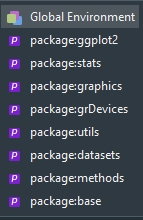
\includegraphics{Captureenvir.PNG}

\end{frame}

\begin{frame}[fragile]{Parametres de fonctions}
\protect\hypertarget{parametres-de-fonctions}{}

\begin{Shaded}
\begin{Highlighting}[]
\NormalTok{a<-}\DecValTok{1}

\NormalTok{fun<-}\ControlFlowTok{function}\NormalTok{(x)\{}
\NormalTok{a<-}\DecValTok{10}
\KeywordTok{return}\NormalTok{(x}\OperatorTok{+}\NormalTok{a)}
\NormalTok{\}}
\KeywordTok{fun}\NormalTok{(}\DecValTok{1}\NormalTok{)}
\end{Highlighting}
\end{Shaded}

\begin{verbatim}
## [1] 11
\end{verbatim}

\begin{Shaded}
\begin{Highlighting}[]
\NormalTok{a}
\end{Highlighting}
\end{Shaded}

\begin{verbatim}
## [1] 1
\end{verbatim}

\end{frame}

\begin{frame}[fragile]{Parametres de fonctions}
\protect\hypertarget{parametres-de-fonctions-1}{}

\begin{Shaded}
\begin{Highlighting}[]
\NormalTok{a<-}\DecValTok{1}

\NormalTok{fun<-}\ControlFlowTok{function}\NormalTok{(x)\{}

\KeywordTok{return}\NormalTok{(x}\OperatorTok{+}\NormalTok{a)}
\NormalTok{\}}
\KeywordTok{fun}\NormalTok{(}\DecValTok{1}\NormalTok{)}
\end{Highlighting}
\end{Shaded}

\begin{verbatim}
## [1] 2
\end{verbatim}

\begin{Shaded}
\begin{Highlighting}[]
\NormalTok{a}
\end{Highlighting}
\end{Shaded}

\begin{verbatim}
## [1] 1
\end{verbatim}

\end{frame}

\begin{frame}[fragile]{Parametres de fonctions}
\protect\hypertarget{parametres-de-fonctions-2}{}

\begin{Shaded}
\begin{Highlighting}[]
\NormalTok{a<-}\DecValTok{1}

\NormalTok{fun<-}\ControlFlowTok{function}\NormalTok{(x)\{}
\NormalTok{a<<-}\DecValTok{10}
\KeywordTok{return}\NormalTok{(x}\OperatorTok{+}\NormalTok{a)}
\NormalTok{\}}
\KeywordTok{fun}\NormalTok{(}\DecValTok{1}\NormalTok{)}
\end{Highlighting}
\end{Shaded}

\begin{verbatim}
## [1] 11
\end{verbatim}

\begin{Shaded}
\begin{Highlighting}[]
\NormalTok{a}
\end{Highlighting}
\end{Shaded}

\begin{verbatim}
## [1] 10
\end{verbatim}

\end{frame}

\begin{frame}[fragile]{Parametres de fonctions}
\protect\hypertarget{parametres-de-fonctions-3}{}

\begin{Shaded}
\begin{Highlighting}[]
\NormalTok{a<-}\DecValTok{1}
\NormalTok{x<-}\DecValTok{100}
\NormalTok{fun<-}\ControlFlowTok{function}\NormalTok{(}\DataTypeTok{x=}\DecValTok{1}\NormalTok{)\{}

\KeywordTok{return}\NormalTok{(x}\OperatorTok{+}\NormalTok{a)}
\NormalTok{\}}
\KeywordTok{fun}\NormalTok{()}
\end{Highlighting}
\end{Shaded}

\begin{verbatim}
## [1] 2
\end{verbatim}

\begin{Shaded}
\begin{Highlighting}[]
\NormalTok{a}
\end{Highlighting}
\end{Shaded}

\begin{verbatim}
## [1] 1
\end{verbatim}

\end{frame}

\begin{frame}[fragile]{Manipuler un environement}
\protect\hypertarget{manipuler-un-environement}{}

\emph{On peut creer et remplir d'autres environements}

\begin{Shaded}
\begin{Highlighting}[]
\NormalTok{a<-}\DecValTok{1}
\NormalTok{env2<-}\KeywordTok{new.env}\NormalTok{()}
\KeywordTok{assign}\NormalTok{(}\StringTok{"a"}\NormalTok{,}\DecValTok{2}\NormalTok{,}\DataTypeTok{envir=}\NormalTok{env2)}

\NormalTok{a}
\end{Highlighting}
\end{Shaded}

\begin{verbatim}
## [1] 1
\end{verbatim}

\begin{Shaded}
\begin{Highlighting}[]
\KeywordTok{get}\NormalTok{(}\StringTok{"a"}\NormalTok{,}\DataTypeTok{envir=}\NormalTok{env2)}
\end{Highlighting}
\end{Shaded}

\begin{verbatim}
## [1] 2
\end{verbatim}

\begin{Shaded}
\begin{Highlighting}[]
\NormalTok{env2}\OperatorTok{$}\NormalTok{b<-}\DecValTok{2}
\NormalTok{env2}\OperatorTok{$}\NormalTok{b}
\end{Highlighting}
\end{Shaded}

\begin{verbatim}
## [1] 2
\end{verbatim}

\end{frame}

\begin{frame}{Interet d'un nouvel environement}
\protect\hypertarget{interet-dun-nouvel-environement}{}

\end{frame}

\end{document}
